% !TeX encoding = UTF-8
% !TeX program = xelatex
% !TeX TXS-program:compile = txs:///xelatex
% !TeX bibtex-program = biber
%
% ============================================================================
%  山东科技大学硕士研究生学位论文开题报告（正文部分）
%  基于 SDUST_Thesis 模板（XeLaTeX + biber 编译）
%  封面 / 评分表 / 评审意见表见 cover.tex（单独编译后与正文合并）
% ============================================================================
%  编译命令（终端）：
%       xelatex main.tex
%       biber main
%       xelatex main.tex
%       xelatex main.tex
% ============================================================================

\documentclass[master]{sdustthesis}  % 选项: master, doctor, bachelor; 可加 review 盲审

\sdustsetup{
  zh/title = {面向发动机燃烧场多组分浓度与关键自由基二维分布同步诊断的激光光谱方法研究},
  en/title = {Laser Spectroscopic Method for Simultaneous Diagnostics of Multi-Component Concentrations and Key Radical Two-Dimensional Distributions in Engine Combustion Fields},
  zh/author = {张洪民},
  en/author = {Hongmin Zhang},
  zh/supervisor = {刘训臣},
  en/supervisor = {Xunchen Liu},
  zh/major = {机械},
  en/major = {Mechanical Engineering},
  zh/department = {机械电子工程学院},
  zh/keywords = {激光燃烧诊断；中红外吸收光谱；平面激光诱导荧光；一氧化氮；同步诊断},
  en/keywords = {Laser combustion diagnostics; Mid-infrared absorption spectroscopy; Planar laser-induced fluorescence; Nitric oxide; Simultaneous diagnostics},
  id = {2024xxxx},
  enrollment = {2024年9月},
  defense = {2027年5月},
  secretlevel = {公开},
  ccode = {TB532},
  udc = {621},
  degreetype = {专业学位},
  degreelevel = {硕士},
  researchfield = {燃烧激光光谱诊断},
  eduduration = {三年},
  graduyear = {2027},
  submitdate = {2027年6月},
  supertitle = {教授},
  reviewers = {匿名评审},
  defensechair = {待定},
  defensecommittee = {待定},
  totalpages = {0},
  fund = {},
  zh/display-date = {二〇二七年六月},
}

% -------- 导言区：自定义宏包和环境（尽量集中管理） ----------
% 代码块环境（基于 listings）
% 注：listings 已在 cls 中加载，无需重复
\lstdefinestyle{mycode}{
  basicstyle   = \ttfamily\small,
  commentstyle = \itshape\color{gray},
  keywordstyle = \bfseries\color{blue},
  stringstyle  = \color{red},
  frame        = single,
  breaklines   = true,
  tabsize      = 4,
  numbers      = left,
  numberstyle  = \tiny\color{gray},
}
\lstnewenvironment{codeblock}[1][]{
  \lstset{style=mycode, #1}
}{}

% 参考文献（使用 biblatex）
\usepackage[backend=biber,style=gb7714-2015,sorting=none]{biblatex}
\renewcommand{\bibfont}{\zihao{5}\setlength{\baselineskip}{16bp}}
\setlength{\bibitemsep}{3bp plus 1pt}
\addbibresource{refs.bib}

% 常用宏包（合并去重）
\usepackage{siunitx}               % 单位
\usepackage{graphicx}
\usepackage{float}                % 图片就地排版 [H]：保证“说明文字→图→图后说明”顺序与 Word 一致
\usepackage{booktabs, multirow, longtable}
\usepackage{bm}                    % 粗体数学符号
\usepackage{amsmath, amssymb}
\usepackage{threeparttable}        % 表格脚注（轻量替代 threeparttablex）
\usepackage{hologo}                % 排版 logo

% 开题报告版式：章/节标题编号与 Word 原文一致（编号写在标题文字里，如"一、立论依据""（1）课题来源…"）
\ctexset{
  chapter = {
    format      = {\centering\zihao{-2}\heiti\bfseries},
    name        = {},
    number      = {},
    beforeskip  = 24pt,
    afterskip   = 24pt,
    fixskip     = true,
  },
  section      = {number = {}},
  subsection   = {number = {}},
  subsubsection= {number = {}},
}

% 页眉：开题报告标题
\RequirePackage{fancyhdr}
\fancypagestyle{sdust@headings}{%
  \fancyhf{}%
  \fancyhead[L]{\zihao{5}\songti 山东科技大学硕士研究生学位论文开题报告}%
  \fancyhead[R]{\zihao{5}\songti \thepage}%
  \renewcommand{\headrulewidth}{0.4pt}%
}

% 图/表编号：全文连续编号（图1、图2…，与开题报告习惯一致）
% 注：ctexbook 默认 figure/table 随章重置，这里撤销重置保证全文连续
\makeatletter
\@removefromreset{figure}{chapter}
\@removefromreset{table}{chapter}
\makeatother
\renewcommand{\thefigure}{\arabic{figure}}
\renewcommand{\thetable}{\arabic{table}}

\begin{document}

% -------- 开题报告正文（封面/评分表单独编译，合并时在前）---------
\mainmatter

% 各章内容
% 第1章 立论依据

\chapter{一、立论依据}

\section{（1）课题来源、选题依据和立论背景}

本课题围绕发动机燃烧场多组分浓度与关键自由基二维分布的同步诊断这一核心科学问题展开。

一氧化氮（NO）是燃烧排放中危害最大、也最难控制的痕量污染物之一：它既是光化学烟雾、酸雨与臭氧层消耗的前体，又是燃烧组织优劣与排放合规程度的直接指示物。在航空发动机、燃气轮机、工业炉窑等实际燃烧装置中，NO 的排放控制长期面临一个共性难题——``看不见、量不准''：火焰内部 NO 的时空分布与绝对浓度难以同步获得，导致减排措施缺乏可靠的定量依据。这一困境具体表现在三个层面：其一，NO 生成机理交织，仿真难以单独支撑。NO 主要通过热力型（Zeldovich 机理，高温区主导）、快速型（Fenimore 机理，火焰前沿）与燃料型（含氮燃料氧化）三条途径生成，其对温度、当量比、停留时间的依赖截然不同，仅靠数值仿真难以准确预测工程装置中的 NO 生成，必须有高时空分辨的实验测量进行判别与验证。其二，传统测量手段难以胜任原位测量。取样法（化学发光、气相色谱）需将气体抽出，破坏流场且响应慢，无法反映瞬态分布；接触式电化学传感器无法承受高温火焰环境，使火焰内部 NO 的分布长期处于``测不到''的状态。其三，现有激光诊断手段各有短板，单一方法难以兼顾成像与定量：激光诱导荧光（PLIF）能给出二维 NO 分布图像，但定量化受荧光猝灭、温度依赖与激光能量衰减等因素制约，标定困难；可调谐激光吸收光谱（TDLAS）能免标定地给出绝对浓度，但只能做视线路径上的积分测量，无法获得空间分布。单一手段始终难以同时满足``看得见''与``量得准''的双重要求，不同系统之间也缺乏可溯源、可相互验证的统一基准。

随着航空发动机、燃气轮机等动力装备向高推重比、低排放方向发展，燃烧室内部温度、组分浓度与反应区结构的精确表征成为燃烧组织优化与排放控制的关键。然而，发动机燃烧场具有高温（可达 2000 K 以上）、高速（湍流脉动微秒量级）、强梯度与强干扰（H$_2$O/CO$_2$ 大量存在）等特征，传统接触式探针（热电偶、取样分析）受响应速度、侵入扰动与寿命限制，难以满足瞬态、非接触、多参数同步测量的要求。激光吸收光谱（TDLAS）与平面激光诱导荧光（PLIF）是当前最具代表性的两类非接触光学诊断手段：前者以高灵敏度、高精度、可定量著称，适合组分浓度与温度的``线/点''测量；后者以高时空分辨、可成场著称，适合火焰结构与自由基``面''分布的瞬态捕捉。二者互补，但受限于可调谐激光器波段覆盖与高能高频光源的可获得性，实现``同一燃烧场内多组分浓度 + 关键自由基分布''的同步测量仍是难点。正是针对上述困境，本课题提出``成像与定量互补、相互验证''的研究思路：以染料激光倍频产生 283 nm 紫外光实现 NO-PLIF 二维成像，以中红外量子级联激光实现 NO 绝对浓度的 TDLAS 定量，二者围绕同一火焰对象交叉标定，建立可溯源的 NO 测量与标定体系。本课题正是基于课题组已有的中红外量子级联激光器（QCL）多通道平台与高频 burst 染料激光平台，围绕上述难点展开，选题具有明确的应用牵引与理论探索价值。

\begin{figure}[H]
  \centering
  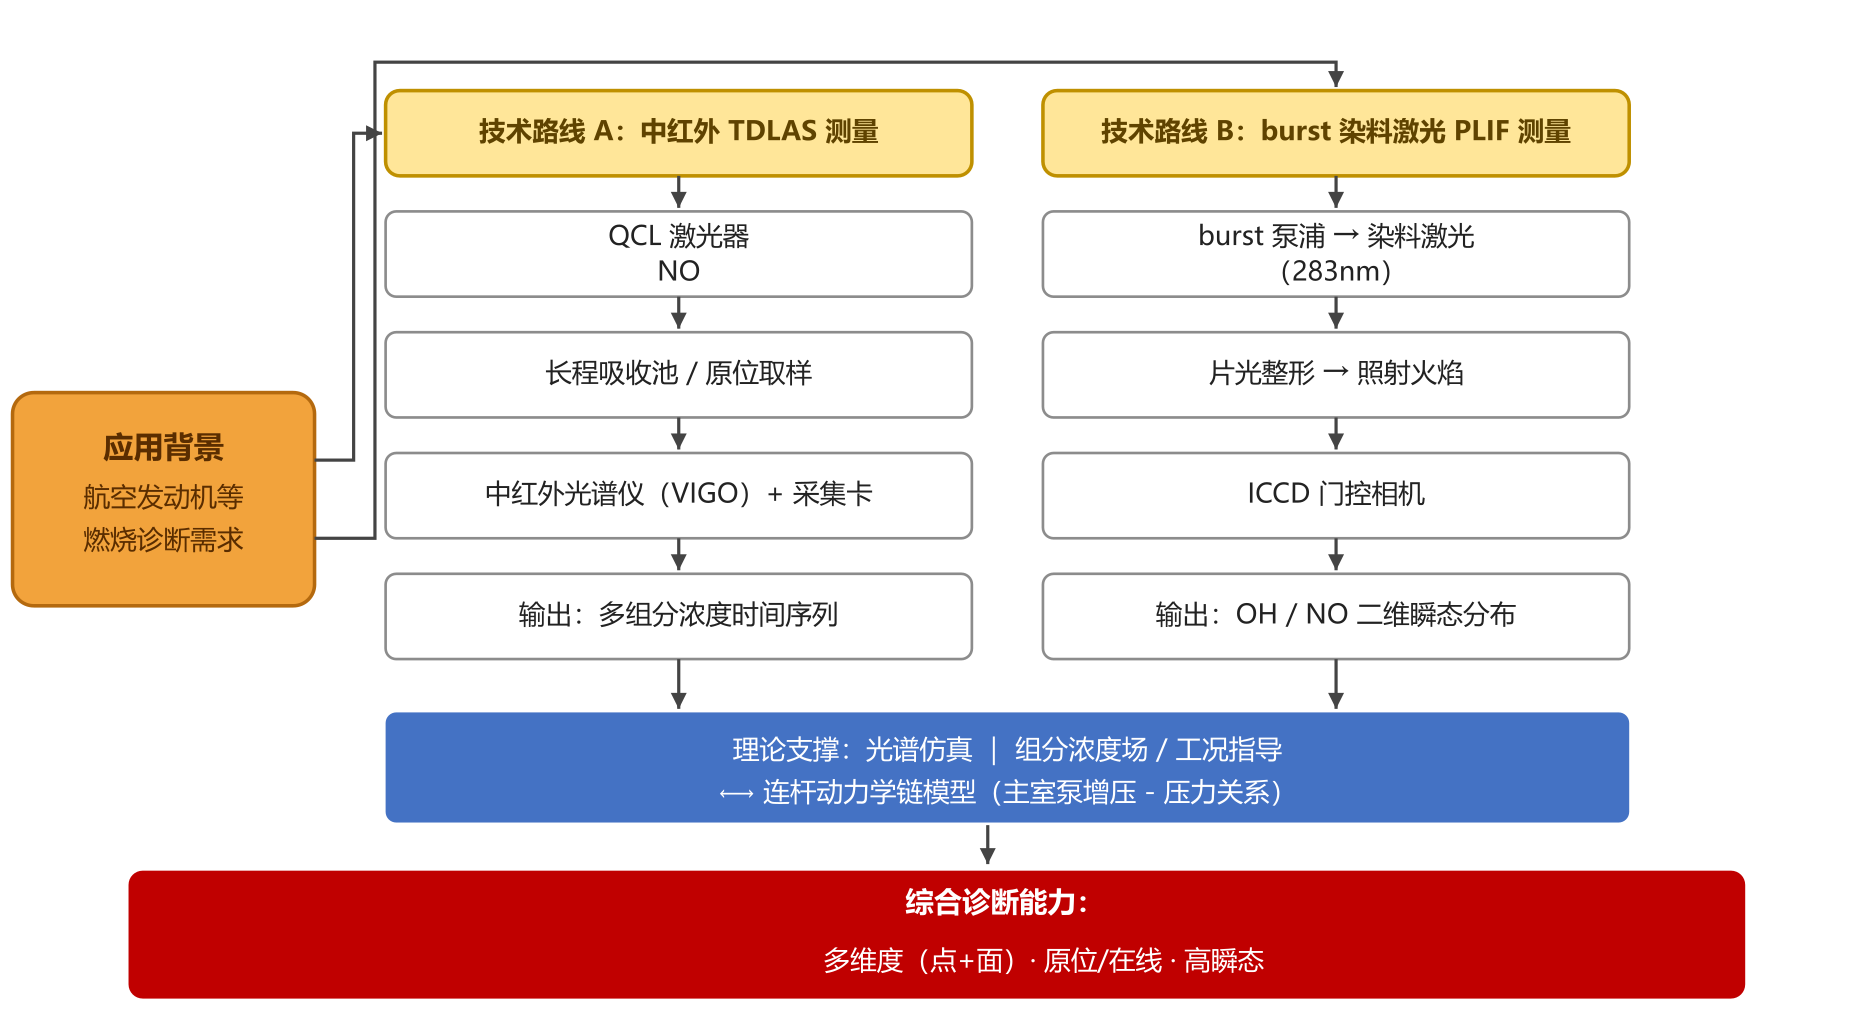
\includegraphics[width=0.85\textwidth]{figures/image1.png}
  \caption{课题总体技术框架：中红外 TDLAS 多组分线测量与 burst 染料激光 NO-PLIF 面测量的协同}
  \label{fig:framework}
\end{figure}

\section{二、课题研究目的、理论意义和实际应用价值}

\subsection{（1）课题研究目的}

本课题以发动机尾气/燃烧场中 NO 的高保真在线诊断与多组分同步诊断为总目标，围绕``定量测量 $\rightarrow$ 二维成像 $\rightarrow$ 手段互校验''三条技术线展开，具体研究目的如下：

（1）建立中红外 QCL-TDLAS 的 NO 在线定量测量方法与浓度反演模型，并同步拓展 CO 通道。面向 NO 5.2 μm 基频带（约 1876 cm$^{-1}$）与 CO 4.6 μm 基频带（约 2143 cm$^{-1}$），开展高温、高压、多组分干扰下的特征谱线筛选与干扰抑制研究；建立基于 Voigt 线型的``吸收谱—温度—浓度''联合反演模型，厘清谱线强度、配分函数、压力展宽与基线抖动等因素对反演误差的传递规律，实现 NO（及同步 CO）浓度的在线、定量、免标定反演。

（2）建立 burst 染料激光泵浦的 NO-PLIF 二维瞬态成像系统，并实现稳定出光与标定。利用 burst 模式染料激光输出 283 nm（NO A$^2\Sigma^+ \leftarrow X^2\Pi$ (0,0) 跃迁）激发 NO 荧光，构建高频脉冲串泵浦的 NO-PLIF 成像光路；攻克染料激光在 burst 模式下的能量稳定性、线宽压窄与频率锁定等关键问题；完成系统的强度—浓度标定，实现 NO 二维浓度场的瞬态、高帧频成像。

（3）探明 QCL-TDLAS 与 NO-PLIF 两种手段在发动机尾气工况下的耦合与互校验机制，形成一体化诊断能力。以 NO 为主线：用 NO-PLIF 的二维分布为 TDLAS 的路径积分反演提供空间均匀性先验、校正``路径平均浓度''与``峰值浓度''的差异；用 TDLAS 的定量浓度反演结果反向校准 NO-PLIF 的强度—浓度标定；建立两者的互校验模型与不确定度传递框架，最终形成``线定量 + 场成像''相互印证的一体化 NO 诊断平台。

\subsection{（2）理论意义}

其一，揭示``线定量—场成像''互补诊断的物理与信息学基础，阐明路径积分浓度与二维浓度场之间的空间映射与权重构造关系，为多手段协同诊断提供理论框架。其二，建立多组分吸收谱（TDLAS）与自由基荧光图像（PLIF）在标准火焰场下的联合标定理论，发展碰撞猝灭、温度—组分依赖与激发效率的统一校正方法。其三，发展高重频 burst 染料激光``高压染料循环稳流 + 蓄能缓冲''的稳定性控制理论，揭示汽蚀抑制、流场均匀性与输出能量抖动的关联机制。其四，构建双向互校验模型与合成不确定度传递框架，推动燃烧激光诊断由``单点/单法''向``可溯源、可互校''演进。

\subsection{（3）实际应用价值}

本课题成果可直接服务于航空发动机、燃气轮机、工业炉窑等动力与能源装备的低排放燃烧组织与 NOx 排放合规：提供可溯源的 NO 在线诊断手段，使减排措施获得可靠的定量依据。所形成的一体化``线定量 + 场成像''诊断能力，可推广至 CO、CO$_2$、N$_2$O 等多组分与 OH 等关键自由基的同步诊断；所搭建的中红外 QCL-TDLAS 与高频 burst 染料激光 PLIF 两套平台，亦可辐射至燃烧、流体与等离子体诊断等相关研究，具有重要的工程应用前景。
          % 第1章 立论依据
% 第2章 文献综述

\chapter{二、文献综述}

\section{1.国内外研究现状、发展动态}

\subsection{（1）激光光源发展}

\subsubsection{染料激光的发展}

国外研究现状。染料激光是最早实现宽带连续可调谐的相干光源之一，自 20 世纪 60 年代中期问世起即成为光谱学与激光化学的主力光源。Duarte 系统梳理了高性能液体与固体窄线宽染料激光振荡器的物理机理与技术体系，指出染料分子宽荧光谱带来的调谐范围优势，与其热透镜效应、三重态吸收、光化学退化等固有限制并存\cite{ref1}；Pavlopoulos 等则从分子结构—光谱性能关联的角度归纳了激光染料的构效关系，为不同波段染料选型提供依据\cite{ref2}。

为克服液体染料的热管理与寿命问题，器件化沿两条路线推进：一条是固体化路线，Duarte 与 James 将染料掺杂聚合物—纳米颗粒复合增益介质引入可调谐固体激光器，在保持调谐能力的同时显著提升光稳定性\cite{ref3}；另一条是分布式反馈（DFB）集成路线，Oki 等利用塑料波导 DFB 结构实现长寿命、高重复频率的染料激光输出\cite{ref4}。泵浦方式也在更新，Burdukova 等报道了半导体激光直接泵浦的可调谐染料激光，摆脱传统 Nd:YAG 或准分子激光泵浦的体积与功耗约束\cite{ref5}。

将染料激光推进到燃烧诊断所需的高重复频率是近年关键进展。Pan 等构建了脉冲串染料激光系统，实现千赫兹重复频率下的高能窄带可调紫外输出，首次把染料激光的宽带调谐能力与脉冲串泵浦的高帧频优势结合起来\cite{ref6}；Mishra 等针对高重复频率脉冲染料激光长期存在的染料池热积累与流场退化问题，用 PIV 对染料池内流场进行表征，指出染料循环与池体结构是高重频下光束质量退化的主控因素\cite{ref7}。

国内研究现状。国内在染料激光本体方向公开报道相对有限，近年有代表性的工作集中在``脉冲串染料激光''这一交叉点上。Chen 等研制了 10 kHz 重复频率、高单脉冲能量的脉冲串染料激光器，系统解决了高重频条件下染料增益介质的热致波前畸变、脉冲串包络均匀性与窄线宽保持问题\cite{ref8}；与之配套，Li 等研制了 10 kHz、10 ns、13.4 mJ 的 Nd:YAG 三倍频脉冲串 MOPA 泵浦源（355 nm），为染料激光提供高重频、高能量的紫外泵浦\cite{ref9}。

\subsubsection{串脉冲（burst-mode）激光器发展}

国外研究现状。脉冲串激光的概念由 Lempert 等在 1996 年提出，其核心思想是用低占空比的短脉冲串替代连续高重频运行，在保持极高瞬时重复频率（可达 MHz）的同时把平均热负载控制在可承受范围\cite{ref10}。随后 Wu 与 Miles 建成 MHz 级高能脉冲串激光系统，并完成激波/边界层干扰的序列可视化\cite{ref11}，标志着该技术进入高速流动诊断实用阶段。

此后发展沿两条主线推进。一是窄线宽化：Thurow 等研制窄线宽 MHz 脉冲串激光器\cite{ref12}，使脉冲串光源可直接服务于需要窄线宽激发的 PLIF 测量，并迭代至第三代系统\cite{ref13}；Jiang 等提出改进的高重频脉冲串输出产生方法，显著改善脉冲串内能量一致性\cite{ref14}。二是能量与时宽扩展：Slipchenko 等实现 100 kHz、100 ms、400 J 的双波长二极管泵浦放大脉冲串激光器\cite{ref15}；Roy 等实现 100 ps 脉宽、100 J 级脉冲串输出以覆盖 kHz--MHz 诊断需求\cite{ref16}；Michael 等把千帧级、100 kHz 的平面成像带入湍流火焰\cite{ref17}；Roy 等进一步提出``三路输出''（three-legged）脉冲串激光架构，实现速度场与多个标量场的同时测量\cite{ref18}。Slipchenko 等在 2021 年燃烧学大会上对脉冲串激光诊断在反应流/非反应流中的进展作了权威综述，明确指出高重频脉冲串泵浦染料激光/OPO 是实现高速自由基成像的关键路径\cite{ref19}；Jiang 等则聚焦高超声速流动场景做了最新总结\cite{ref20}。

国内研究现状。国内以哈尔滨工业大学（陈德应、李旭东、闫仁鹏、于欣等）为主的团队已形成较完整的脉冲串激光技术链。闫仁鹏等采用 YAG/Nd:YAG/Cr$^{4+}$:YAG 复合晶体实现高重频、高峰值功率脉冲串输出\cite{ref21}；吴文韬等通过增益分布控制的侧面泵浦实现平顶光束输出的腔倒空脉冲串 MOPA 系统\cite{ref22}；近年工作进一步向高重频、窄线宽、包络整形方向发展，于欣等实现 100 kHz 窄线宽、包络均匀的脉冲串 MOPA 系统\cite{ref23}，徐浩波等在 2025 年用变反射率非稳腔进一步优化高重频脉冲串 Nd:YAG 输出\cite{ref24}。

如图 2 为脉冲串激光产生原理，图 3\cite{ref25} 为染料激光从 1963—2019 年的发展历史。从图中可以看出：单次 burst 内脉冲数量（绿色 M）持续增加，从早期几个脉冲发展到单次 burst 上百个脉冲，支持更多帧连续 PLIF 图像；脉冲串持续时间不断拉长，从 0.1 ms 发展到数 ms、最长可达 30 ms，给湍流火焰更长的高速观测窗口；重复频率（蓝色 f）与单 burst 总能量同步提升，既能做到 kHz/MHz 高频子脉冲，又保留足够高的脉冲能量，满足紫外倍频做 NO-PLIF 的能量需求。

\begin{figure}[H]
  \centering
  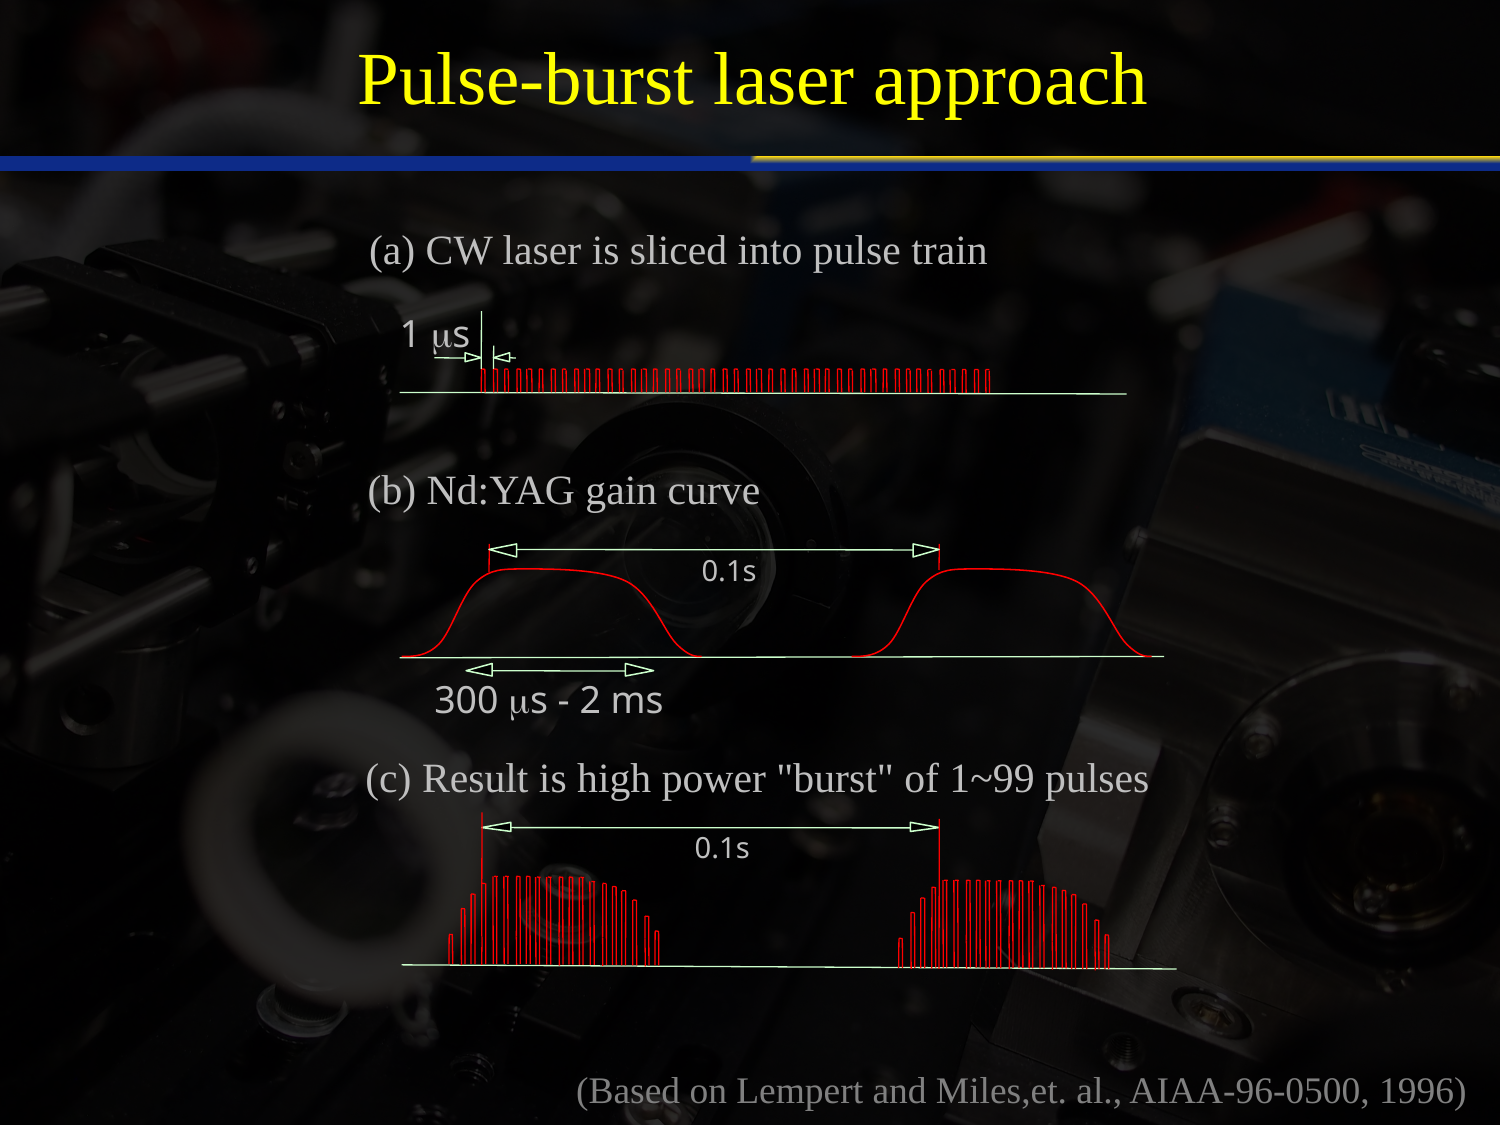
\includegraphics[width=0.75\textwidth]{figures/image2.png}
  \caption{Pulse-burst 激光产生原理}
  \label{fig:burst-principle}
\end{figure}

\begin{figure}[H]
  \centering
  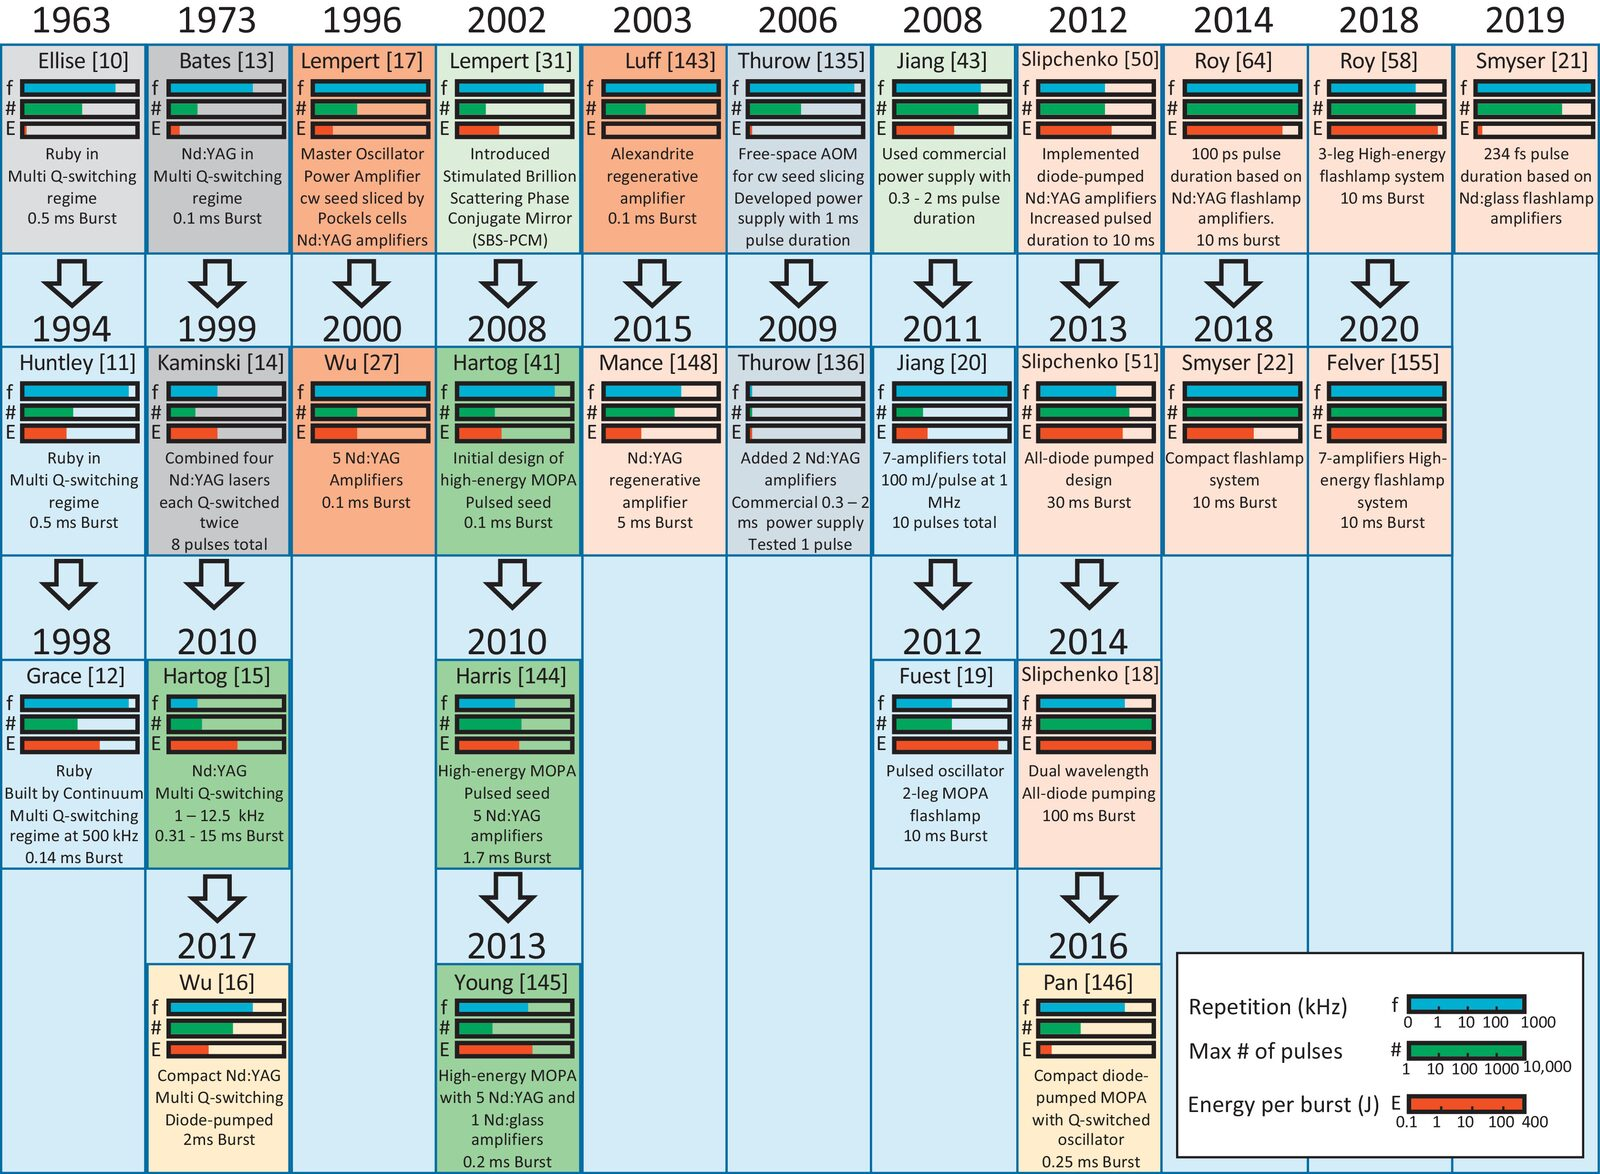
\includegraphics[width=0.85\textwidth]{figures/image3.jpeg}
  \caption{burst 染料激光发展历程}
  \label{fig:burst-history}
\end{figure}

\subsection{（2）PLIF（平面激光诱导荧光）发展}

\subsubsection{国外研究现状}

PLIF 由点测量 LIF 发展而来：Ald\'{e}n 等 1982 年用二极管阵列探测器获得大气火焰中 OH 荧光的单脉冲空间分辨图像\cite{ref26}；Allen 等随后用 CH 与 C$_2$ 的 PLIF 对碳氢—空气火焰反应区进行数字成像，标志着 PLIF 成为燃烧二维成像的主流手段\cite{ref27}。

定量化是长期难点，核心是碰撞猝灭。Tamura 等系统测定了低压碳氢火焰中 CH(A)、OH(A)、NO(A) 的碰撞猝灭规律\cite{ref28}，为荧光信号的温度与组分依赖校正提供了物理基础；此后围绕 NO(A$^2\Sigma^+$) 与 O$_2$、H$_2$O 等非反应/反应碰撞猝灭动力学的成像研究持续推进。这一物理机制决定了：PLIF 给出的是``相对荧光强度分布''，要转化为绝对浓度必须解决猝灭速率的温度—组分依赖与激发效率标定问题。

高重复频率化是 PLIF 近二十年的主旋律。Jiang 等实现 500 kHz 帧频的 NO-PLIF 成像\cite{ref29}，并在 CUBRC 48 英寸激波风洞完成 NO-PLIF 流场成像；Hammack 等在 10 kHz 下对 seeded 流场、等离子体放电与火焰中的 NO 进行 PLIF 测量\cite{ref30}；在 OH/CH$_2$O 等组分的高速成像与多参量同步方面，Wang 等实现湍流火焰中多组分同步超高速 PLIF 成像\cite{ref31}，Halls 等用脉冲串体激光诱导荧光获得燃烧中间组分的四维时空演化\cite{ref32}，Hsu 等在旋转爆震燃烧室中实现 MHz 级 OH-PLIF 成像\cite{ref33}，Hammack 等把 20 kHz CH$_2$O/OH-PLIF 与立体 PIV 同步。针对高重频 NO-PLIF 的光源瓶颈，Leonov 等对用于高重频 NO-PLIF 的光参量振荡器（OPO）进行优化设计\cite{ref34}，Rodrigues 等实现 100 kHz 高光谱分辨率 NO-PLIF 测量\cite{ref35}。

Wang 等用单台染料激光同时成像氨—氢—氮火焰中的 NO 与 NH\cite{ref36}；Chatelain 等用单台染料激光实现 NO 与 OH 的同时 PLIF\cite{ref37}；Wang 等进一步实现 NH$_3$、NH、NO 三组分的同时测量\cite{ref38}；Tang 等把 NH/NO 同步 PLIF 用于等离子体助燃氨/氢旋流火焰。这些工作证明了染料激光在 NO-PLIF 中的独特价值——宽带调谐使一台染料激光即可覆盖多个自由基的激发线，正好呼应前文``脉冲串染料激光''的发展方向，也为``一台光源、多组分同步成像''提供了直接的技术范式。

\subsubsection{国内研究现状}

国内 PLIF 研究起步稍晚但发展迅速。陈爽等提出火焰中瞬时二维 OH-PLIF 测温的标定方法\cite{ref39}；刘训臣等用双波长切换的脉冲串激光实现单相机 20 kHz 双色甲醛 PLIF 测温\cite{ref40}；在超燃冲压方向，王林森等用 acetone-PLIF 研究燃烧室燃料/空气掺混特性，万明罡等提出在强火焰自发光背景下实现瞬时 CH$_2$O-PLIF 成像的策略，汪洪波等用高速相机与双组分 PLIF 同步技术可视化超声速燃烧\cite{ref41}；在旋流燃烧方向，尹盛铭等对双级径向旋流燃烧室的火焰形态转变进行了激光诊断研究。

\section{（3）现有研究的不足与本课题切入点}

综合上述文献，现有研究仍存在以下不足，构成本课题的切入点：

（1）多组分 TDLAS 与自由基 PLIF 多为独立系统，缺乏同一标准场下的交叉校验与一体化标定；

（2）中红外 QCL 与 burst 染料激光共用时序、触发与数据采集的同步机制尚不成熟；

（3）burst 染料激光在高电感/高频工况下的稳定性（能量抖动、线宽展宽、波长漂移）控制缺乏系统研究。

发展趋势：由单组分向多组分、由近红外向中红外、由离线标定向原位在线、由单点向多线/断层成像演进。本课题正是在这一趋势下，围绕``线定量 + 场成像''一体化诊断展开。

\section{所阅文献的查阅范围及手段；参考资料}

参考资料（所阅主要文献）：

\printbibliography[heading=none]
          % 第2章 文献综述（含"所阅文献的查阅范围及手段；参考资料"节内参考文献列表）
% 第3章 研究内容、技术路线、创新点

\chapter{三、研究内容、技术路线、创新点}

\section{（1）主要研究内容}

\subsection{1）中红外通道吸收池光路联调与浓度反演精度验证}

围绕四通道中红外 QCL-TDLAS 平台，拟重点突破折返式吸收池光路（原位反射框架）的装调与``吸收谱—温度—浓度''联合反演的精度验证：（1）完成反射镜组排布、光轴对准与有效光程标定，解决窗口污染引起的透过率漂移补偿与光束抖动对反演稳定性的影响；（2）基于 Voigt 线型前向模型，由双线线强比或 H$_2$O 通道确定温度、以非线性最小二乘反演各组分浓度，系统评估谱线强度、配分函数、压力展宽系数、基线漂移与光程标定误差对反演结果的传递规律，给出各通道的浓度不确定度预算；（3）结合 Cantera 一维火焰仿真完成浓度/温度标定，并在不同当量比、不同停留时间下考察模型的外推能力与高温高压工况下的反演精度（目标：实验—仿真偏差 $<$ 20\%）。

\subsection{2）探明 QCL-TDLAS 与 NO-PLIF 两种手段在发动机尾气工况下的耦合与互校验机制，形成一体化诊断能力}

针对多组分 TDLAS 与自由基 PLIF 长期各自独立、缺乏同一标准场下交叉校验的问题，拟建立两者的耦合与互校验机制：

（1）以统一主时钟/触发源同步 QCL 波长扫描时序、burst 染料激光脉冲串与高速相机曝光时序，实现``同一时刻、同一区域''的同步测量；

（2）利用多程吸收光路与片光的几何对应关系，把 TDLAS 路径积分浓度映射到 PLIF 二维浓度场，由 PLIF 提供空间均匀性先验以校正``路径平均浓度''与``峰值浓度''差异，反向以 TDLAS 免标定结果为 PLIF 强度—浓度标定提供基准，形成双向互校验；

（3）在标准火焰与发动机尾气工况下建立互校验模型与合成不确定度框架，最终形成``线定量 + 场成像''相互印证的一体化 NO 诊断能力。

\section{拟采取的研究方法、技术路线、实施方案及可行性分析}

\subsection{（1）研究方法}

本课题采用``仿真选线—平台搭建—标准场标定—现场验证''的研究方法：首先以 HITRAN/HITEMP 仿真与 Cantera 一维火焰计算确定谱线与工况；其次并行搭建中红外 QCL-TDLAS 与 burst 染料激光 PLIF 两套平台；随后在标准火焰台完成标定；最后在地面试验台/发动机尾气工况下开展现场测量与交叉校验，并对实验—仿真偏差进行校正。

\subsection{（2）技术路线与实施方案}

\subsubsection{1）技术路线}

本课题采用``仿真选线—平台搭建—标准场标定—现场验证''的技术路线：首先以 HITRAN/HITEMP 仿真与 Cantera 一维火焰计算确定谱线与工况；其次并行搭建中红外 QCL-TDLAS 与 burst 染料激光 PLIF 两套平台；随后在 Hencken 标准火焰台完成标定；最后在地面试验台/发动机尾气工况下开展现场测量与交叉校验，并对实验—仿真偏差进行校正。

\subsubsection{2）实施方案}

阶段一：仿真与选线。基于 HITRAN/HITEMP 与自编 Voigt 程序筛选 NO 目标谱线，用 Cantera（GRI-Mech 3.0）一维 Hencken 火焰计算目标工况的温度/物种分布，为选线与反演提供先验。

阶段二：TDLAS 平台搭建（结构设计 + 联调）。完成 QCL 发射—探测、折返式长光程吸收池（原位反射框架）装调与有效光程标定、波长扫描与联合反演算法，结合 Cantera 完成浓度/温度标定与误差评估。

阶段三：PLIF 平台搭建（结构设计 + 联调）。完成染料激光泵浦—振荡光路、高压染料循环/蓄能系统（染料循环泵系统制作）、283 nm 片光与高速相机采集；攻克 burst 模式能量稳定性、线宽压窄与频率锁定，完成强度—浓度标定。

阶段四：点—面协同与交叉校验。统一时序触发，在标准火焰与发动机尾气工况下开展 TDLAS 与 PLIF 交叉比对、偏差校正与不确定度合成，形成一体化诊断能力。

\subsection{（3）可行性分析}

\subsubsection{1）理论和技术可行}

以 Voigt 线型为前向模型的``吸收谱—温度—浓度''联合反演、PLIF 荧光猝灭校正、标准火焰标定等均有成熟物理基础与大量文献支撑；burst 染料激光与 QCL 技术已工程化；本课题提出的``线定量 + 场成像''互校验架构在物理与信息学上自洽，理论可行。中红外 QCL 四通道激光器与 burst 染料激光平台均已到位，关键技术路线清晰。

\subsubsection{2）实验条件可行}

课题组已具备：中红外 QCL 通道激光器（NO）与 VIGO 中红外探测器（已验收）；HITRAN/HITEMP + 自编 Voigt 仿真代码、Cantera 一维火焰仿真；染料泵系统、高速相机、片光源等已到货；既有激光诊断平台。关键仪器与经费基本到位，实验条件可行。

\section{论文的创新点}

（1）提出``中红外多组分 TDLAS 线测量 + burst 染料激光自由基面测量''的协同诊断架构，实现同一燃烧场内浓度与结构的同步表征。

（2）针对 burst 模式下染料激光能量抖动与线宽展宽问题，发展高压染料循环稳流与蓄能缓冲相结合的稳定性控制方法（染料循环泵系统与蓄能缓冲设计）。

（3）建立多组分吸收谱线与 PLIF 自由基图像在标准火焰场下的联合标定与交叉校验方法，形成``线定量 + 场成像''相互印证的一体化 NO 诊断能力——即探明 QCL-TDLAS 与 NO-PLIF 在发动机尾气工况下的耦合与互校验机制。
          % 第3章 研究内容、技术路线、创新点
% 第4章 前期基础工作

\chapter{四、前期基础工作}

\section{1）结构设计}

a. 中红外 QCL-TDLAS 折返式长光程原位测量光路（含原位反射框架制作）如图 4 所示。四通道中红外 QCL 激光器与中红外探测器布置在试验段的同一侧，激光经试验段两侧壁面反射镜组在流场中多次折返后由探测器接收，气流穿过光路区。折返式（多程）结构在不加大装置尺寸的前提下把有效吸收光程提高数倍，使 ppm 量级 NO 的积分吸光度由``难以分辨''提升到``可稳定反演''；多程光路被约束在同一测量截面附近，与下游 PLIF 面测量处于同一测量区域，为两种手段的交叉校验提供几何一致性。该部分的具体研究内容包括反射镜组排布与光轴对准（即原位反射框架的制作与装调）、有效光程长度标定、窗口污染引起的透过率漂移补偿，以及激光光束抖动对反演稳定性的影响。

\begin{figure}[H]
  \centering
  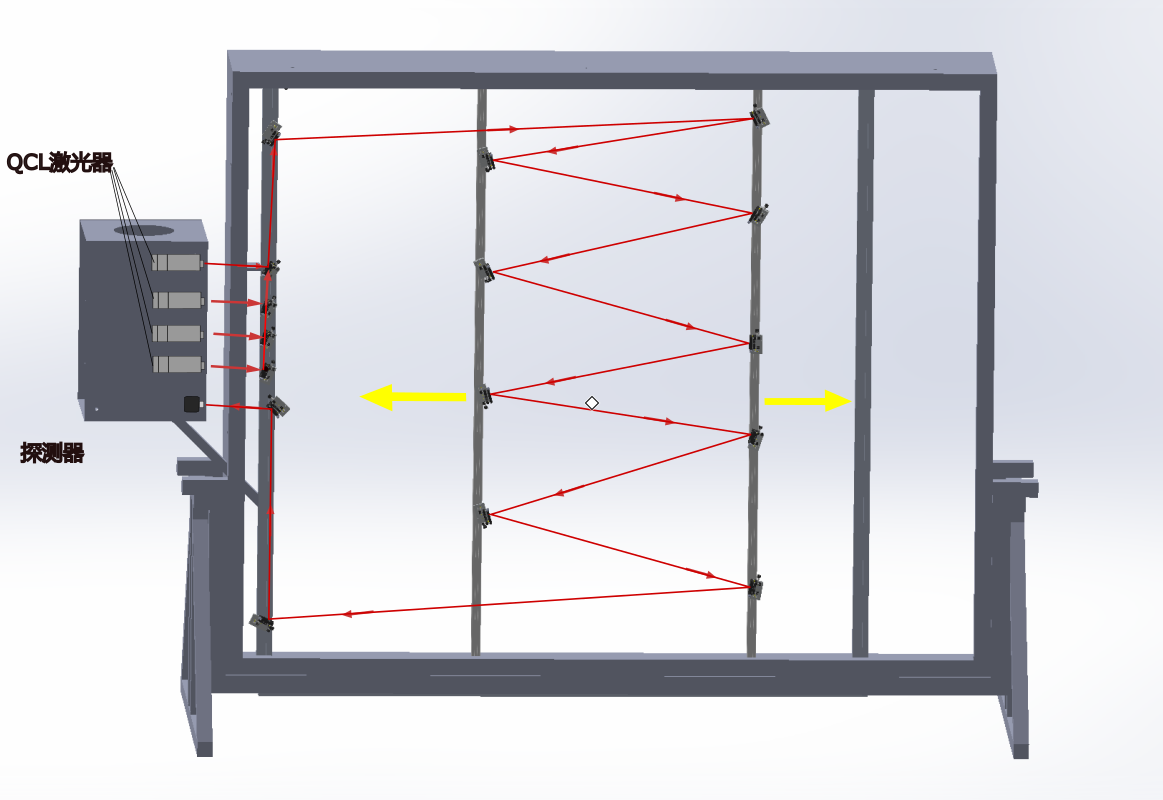
\includegraphics[width=0.85\textwidth]{figures/image4.png}
  \caption{原位测量试验台}
  \label{fig:test-rig}
\end{figure}

b. 染料激光光路与高压染料循环/蓄能缓冲系统（含染料循环泵系统制作）如图 5—8 所示。Nd:YAG 泵浦激光输出 1064 nm 基频，经 KTP 晶体倍频产生 532 nm 绿光，二向色镜滤除残余 1064 nm 后，由 $\lambda/2$ 半波片与格兰棱镜调节偏振态与能量，再经转向镜与聚光透镜耦合进入 Rh6G 染料池；染料激光在``扩束型光栅 + 输出耦合镜''构成的振荡腔内实现 560--650 nm 连续可调谐输出，最后经 BBO 晶体倍频、Pellin-Broca 棱镜分光，得到 283 nm 紫外输出。

\begin{figure}[H]
  \centering
  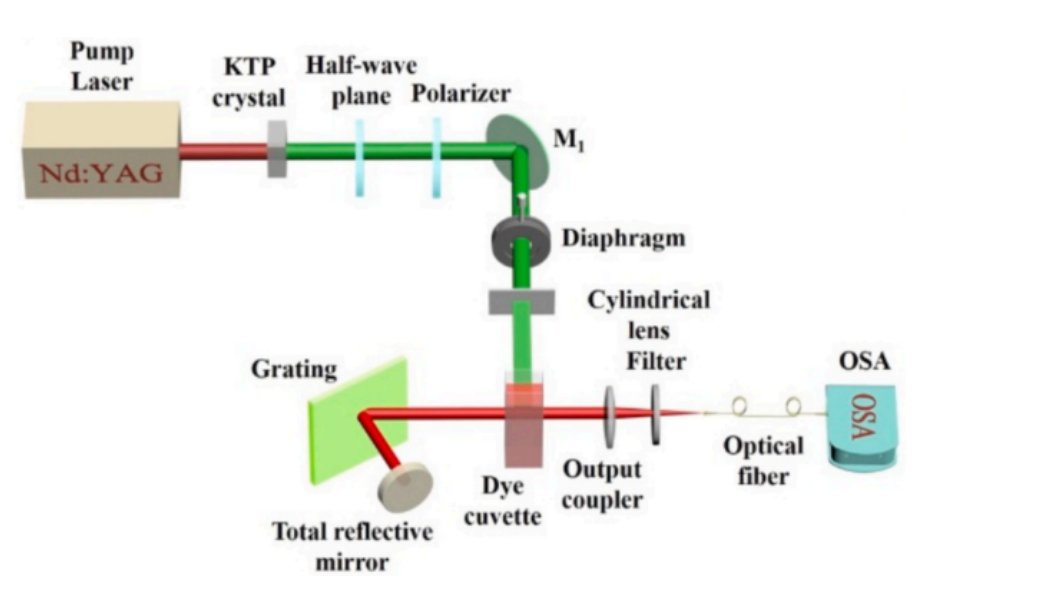
\includegraphics[width=0.75\textwidth]{figures/image5.png}
  \caption{染料激光工作示意图}
  \label{fig:dye-schematic}
\end{figure}

\begin{figure}[H]
  \centering
  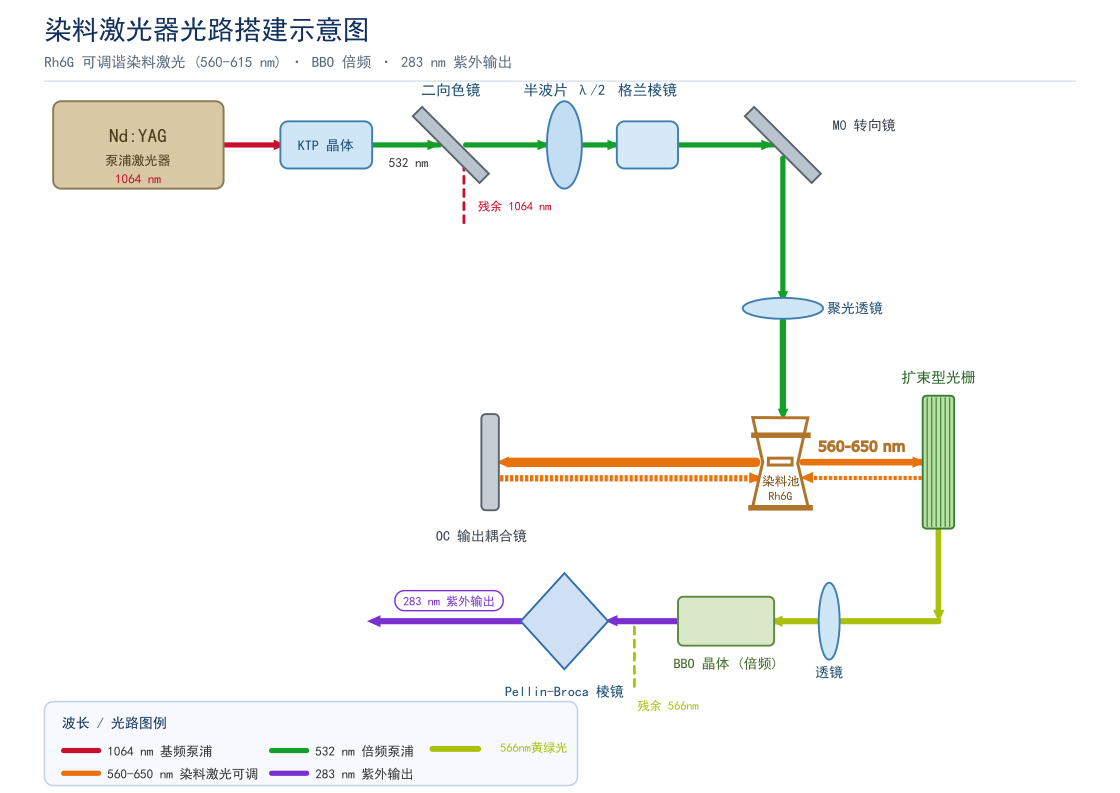
\includegraphics[width=0.85\textwidth]{figures/image6.png}
  \caption{染料激光器光路搭建示意图}
  \label{fig:dye-optical-path}
\end{figure}

高重频下染料池内的热积累与汽蚀是光束质量退化的主控因素，为此设计高压染料循环与蓄能缓冲系统（染料循环泵系统制作）如图 7 所示，是系统整体示意图。图 8 所示是染料泵装置实物图：介质罐中的染料经球阀、齿轮泵/柱塞泵、单向阀与针阀进入液压缸，再经三路单向阀与观察窗回流至泵前构成闭式循环；氮气瓶经减压阀、高压球阀与控压针阀向液压缸加压，形成增压与蓄能缓冲支路，以高压蓄能缓冲抑制汽蚀、稳定流场，把高重频下的能量抖动与波前畸变控制在可接受范围内。回路中布置压力传感器、压力表与观察窗用于实时监测染料压力与流场脉动，气动电磁阀与安全阀承担快速卸压与超压保护功能。

\begin{figure}[H]
  \centering
  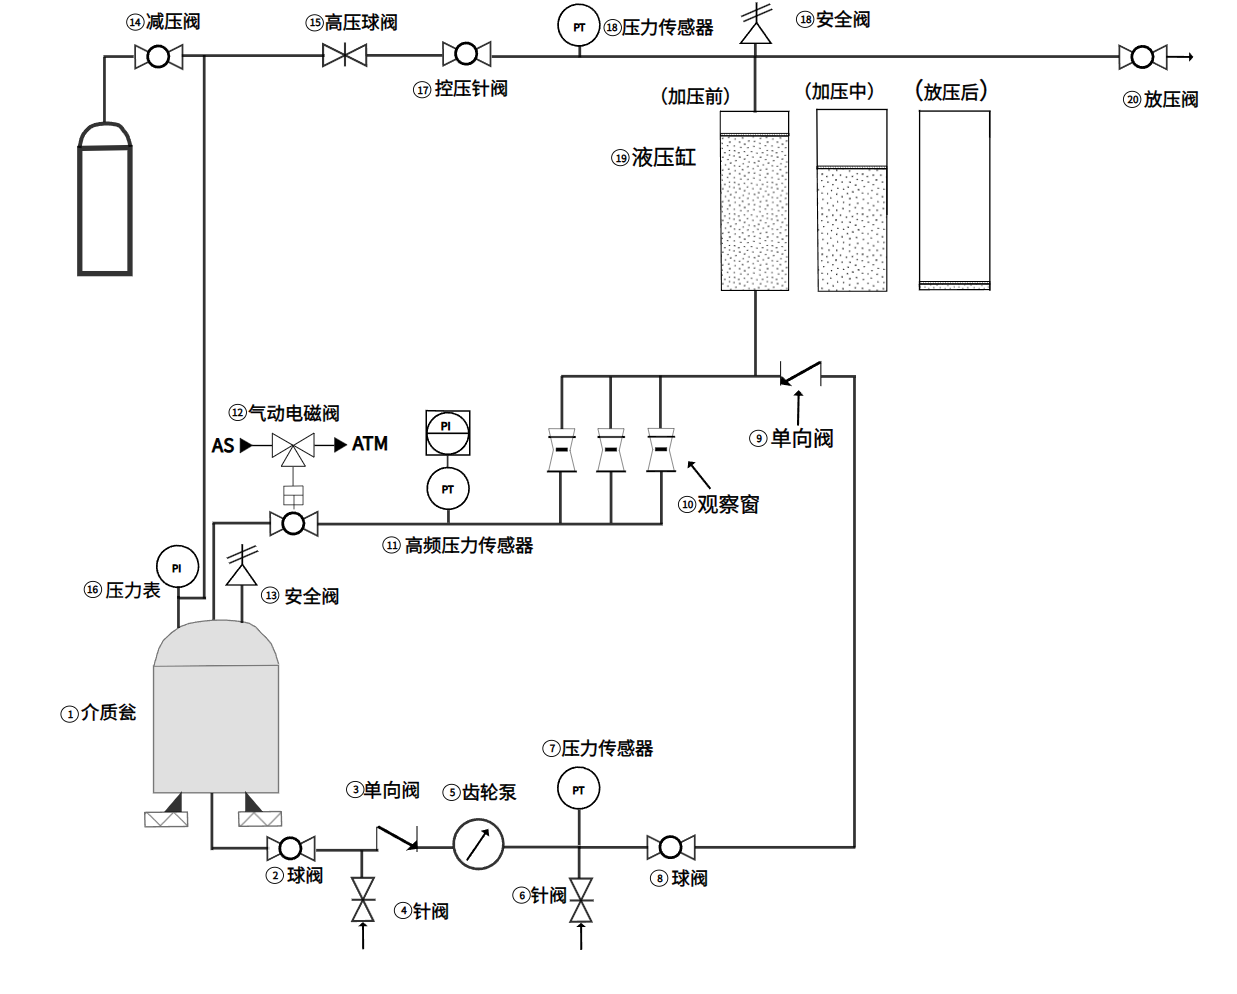
\includegraphics[width=0.85\textwidth]{figures/image7.png}
  \caption{染料泵循环系统示意图}
  \label{fig:dye-pump-system}
\end{figure}

\begin{figure}[H]
  \centering
  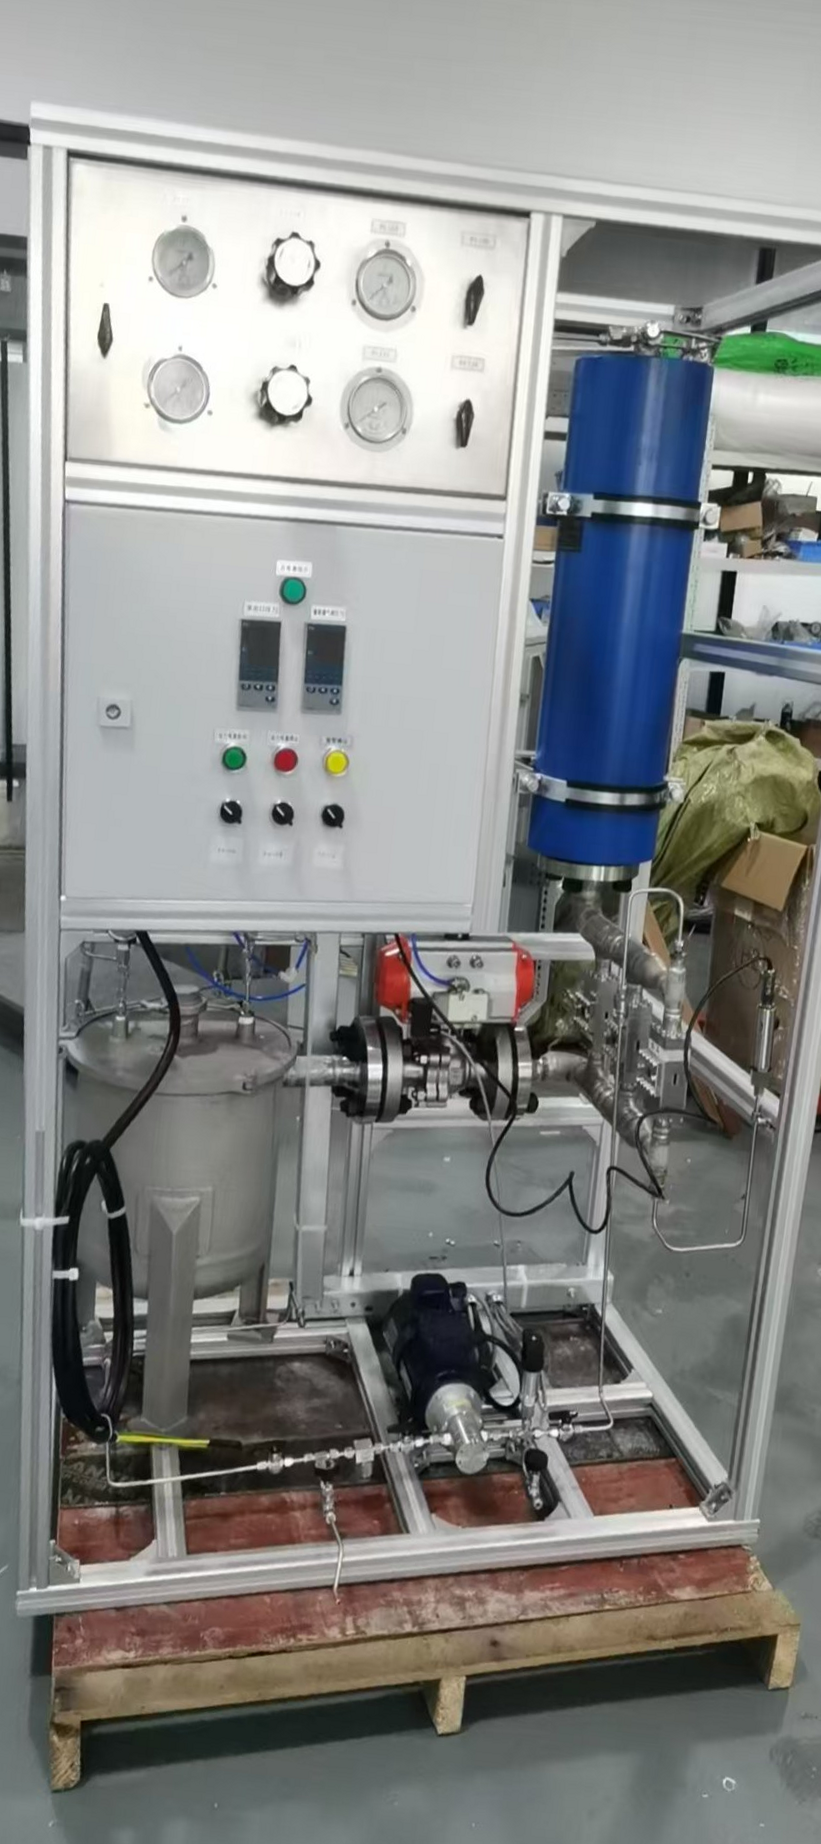
\includegraphics[width=0.35\textwidth]{figures/image8.png}
  \caption{染料泵装置实物图}
  \label{fig:dye-pump-photo}
\end{figure}

\section{2）试验研究}

a. 中红外 QCL-TDLAS 多组分在线测量试验。基于 HITRAN/HITEMP 数据库与自编 Voigt 线型程序，为目标工况优选 NO（5.2 μm）谱线，确保通道正常正常工作；搭建中红外 QCL 发射—探测系统，开展波长扫描与``吸收谱—温度—浓度''联合反演算法研究；结合 Cantera 一维火焰仿真完成测量结果的浓度/温度标定与误差评估。

如图 9 所示的是常见的空气常见的集中气体分子在不同温度下的吸收表现，图 10 则是 NO 在不同温度下的吸收表现。在 NO 探测波长的选取上，本文以其振转基频带（$v = 1 \leftarrow 0$，X$^2\Pi$，中心波数约 1876 cm$^{-1}$）所在的中红外 5.2--5.3 μm 区域为基础，多组分光谱仿真结果，将 NO 探测窗口选定为 1894--1914 cm$^{-1}$，主要依据如下：其一，该窗口覆盖 NO 基频带 R 支中段（R(4)--R(10) 附近），谱线强度位居整个谱带前列，吸光度充足且可选谱线数量多，便于筛选低干扰目标线；其二，由光谱仿真可见，CO$_2$ 与 CO 的吸收集中于 1894--1904 cm$^{-1}$，而 1900--1910 cm$^{-1}$ 附近 H$_2$O 谱线密度显著降低，NO 吸收在该子区间占主导，且窗口上沿之外（$>$1914 cm$^{-1}$）H$_2$O 谱线重新变得密集，故该窗口是保证 NO 线强度前提下干扰最小的折中选择；其三，该窗口在 300--1300 K 全温区范围内均保持可观的 NO 吸收强度，兼顾常温标定与高温燃烧在线测量需求，并可在同一窗口内选取两条低态能量不同的谱线实现双线法测温；其四，5.2--5.3 μm 波段光源（DFB-QCL、OPO 等）与探测器（热电制冷 MCT、VIGO 光伏探测器等）技术成熟，无紫外波段的深紫外光源损伤风险、火焰化学发光与强散射背景，并与课题组既有中红外吸收光谱探测体系兼容。综上，1894--1914 cm$^{-1}$ 是兼顾谱线强度、干扰水平、温度适应性与工程可实现性的 NO 优选探测窗口。

\begin{figure}[H]
  \centering
  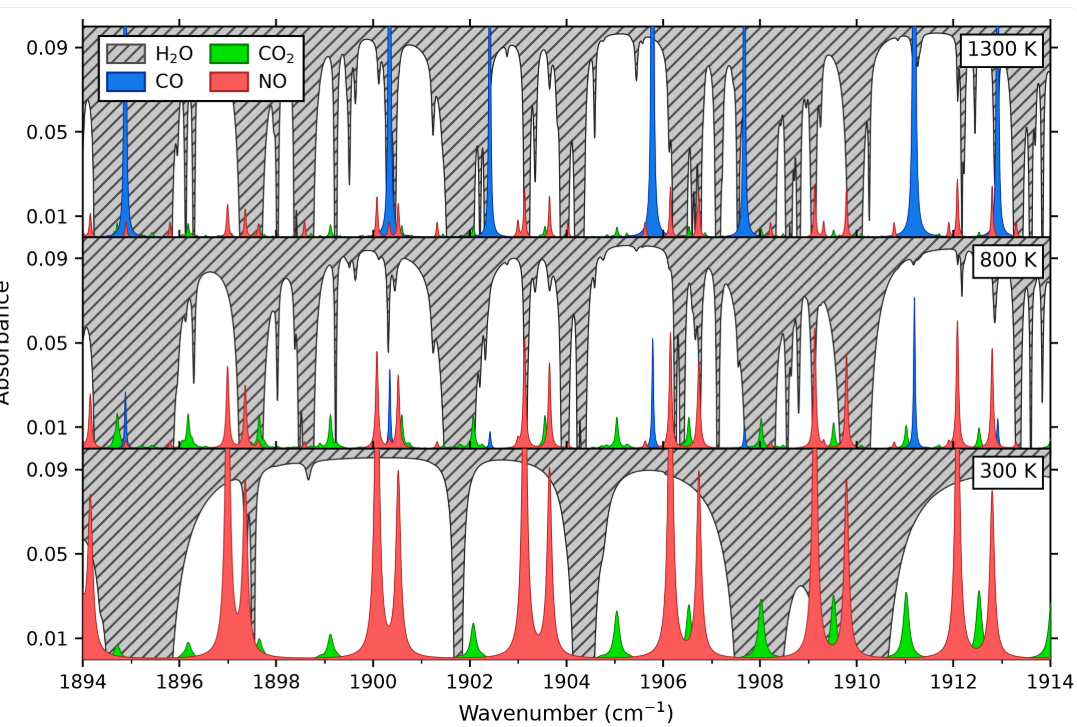
\includegraphics[width=0.85\textwidth]{figures/image9.png}
  \caption{四组分中红外吸收光谱温度特性（300 / 800 / 1300 K）}
  \label{fig:four-species-temp}
\end{figure}

\begin{figure}[H]
  \centering
  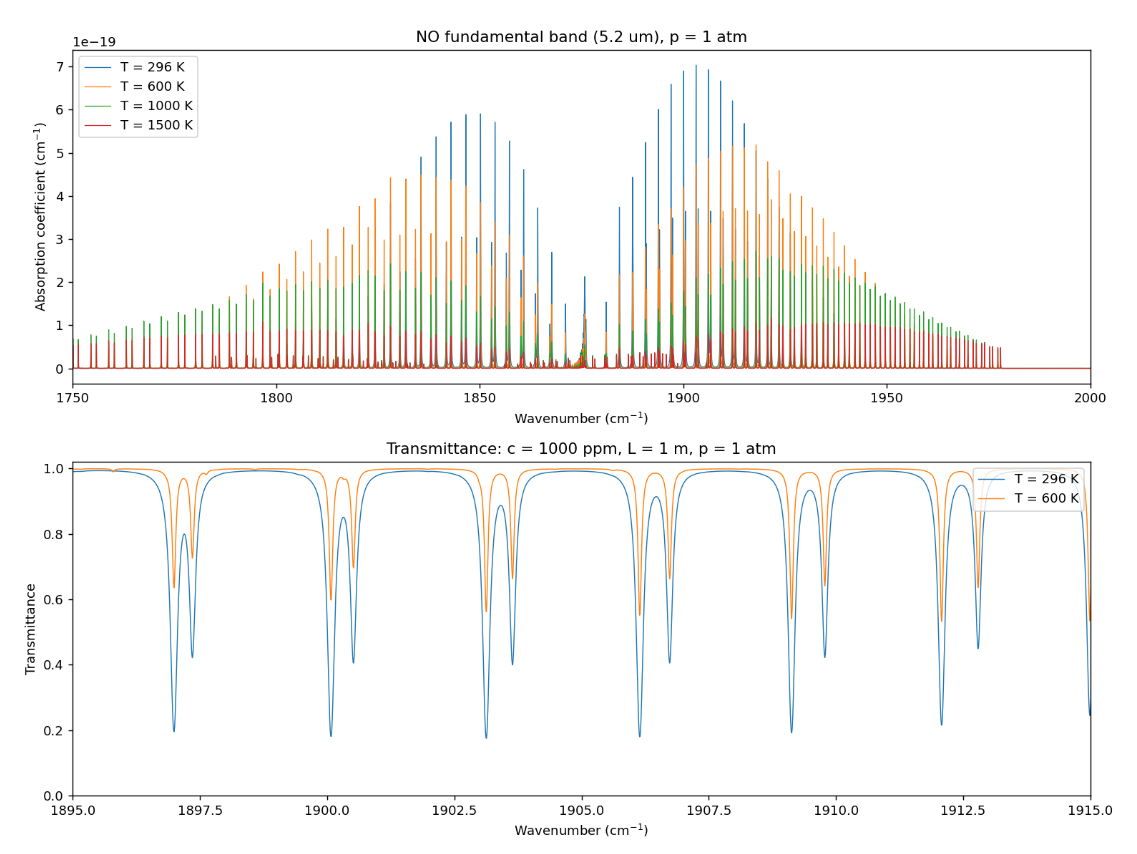
\includegraphics[width=0.8\textwidth]{figures/image10.png}
  \caption{NO 红外吸收光谱温度特性（1750--2000 cm$^{-1}$）}
  \label{fig:no-temp}
\end{figure}

\begin{figure}[H]
  \centering
  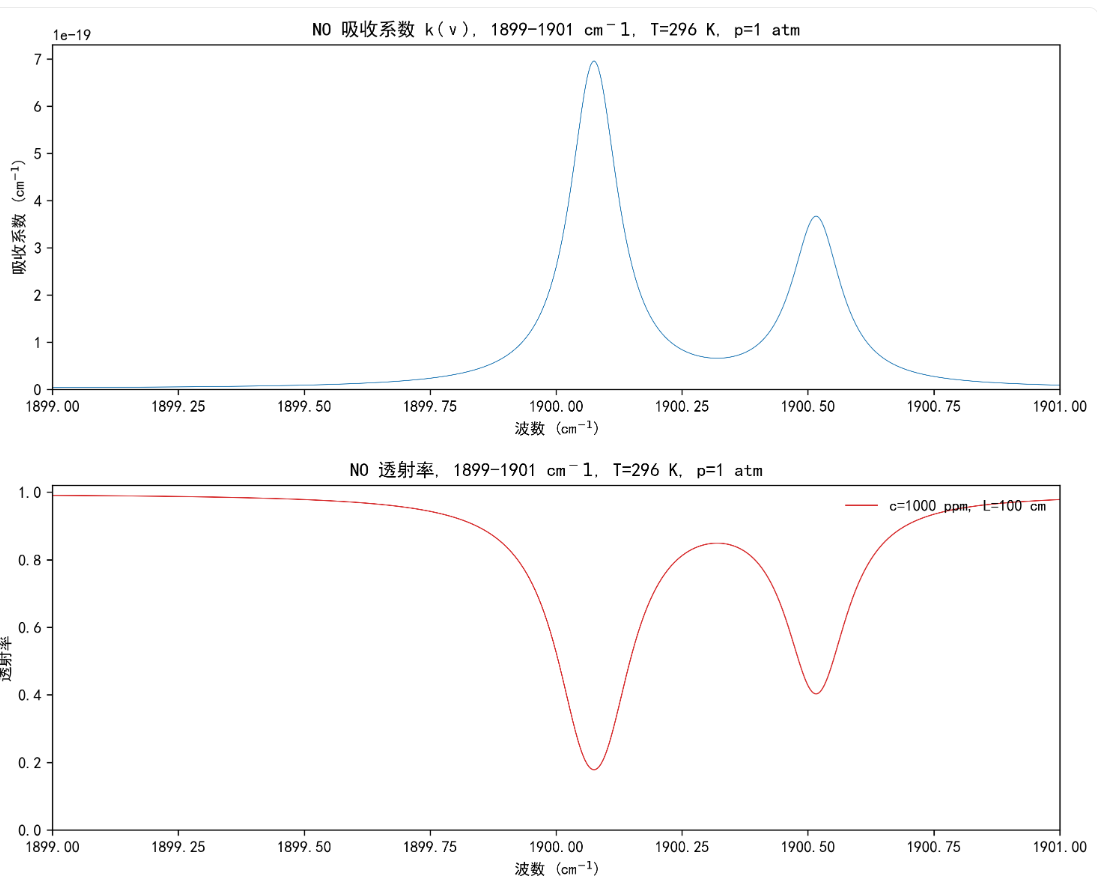
\includegraphics[width=0.8\textwidth]{figures/image11.png}
  \caption{NO 在 1900 cm$^{-1}$ 的吸收系数及透射率}
  \label{fig:no-1900}
\end{figure}

如图 11 所示，为 NO 在 1899--1901 cm$^{-1}$ 窄波段的吸收特性仿真结果。上图为该波段的吸收系数 $k(\nu)$ 分布，下图为对应典型测量工况（$c$ = 1000 ppm，$L$ = 100 cm，$T$ = 296 K，$p$ = 1 atm）下的透过率谱，两图横轴一致，分别反映谱线的固有吸收强度与实际可测信号。

由吸收系数谱可见，该波段内存在两条彼此分离的强吸收线，分别位于 1900.08 cm$^{-1}$ 与 1900.50 cm$^{-1}$。谱线呈典型 Lorentz 线型：296 K、1 atm 下多普勒展宽仅约 0.004 cm$^{-1}$，远小于压力展宽，Voigt 线型可近似为 Lorentz 线型；谱线半高全宽约 0.2 cm$^{-1}$，两线间距 0.42 cm$^{-1}$ 大于谱线半宽，因此可清晰分辨，但线翼仍存在一定重叠，定量反演时需考虑两线的相互贡献。

由透过率谱可见，在 1000 ppm 浓度、100 cm 光程条件下，两条谱线中心的透过率分别降至约 21\% 与 42\%，对应吸光度（$A = -\ln T$）约 1.56 与 0.87。这表明所选谱线在典型燃烧场浓度与光程条件下具有充足的吸收深度，可为直接吸收光谱或波长调制光谱测量提供足够的信噪比；同时也说明在 1000 ppm 高浓度工况下吸收已接近饱和区（$A > 1$）。

综上，该窄波段仿真验证了前文谱线优选的结果：上述两条强线位于 1900 cm$^{-1}$ 附近 H$_2$O 干扰相对最弱的区间，吸收深度适中，可作为 NO 浓度反演的目标谱线。

b. 高频 burst 染料激光 OH/NO-PLIF 成像试验。构建 burst 脉冲串泵浦的片光成像光路，配合高速相机开展 OH/NO-PLIF 二维瞬态测量；研究 burst 模式下染料激光输出稳定性（能量抖动、线宽展宽、波长漂移）及其对 PLIF 信号定量性的影响；以 283 nm 紫外片光照射测量区，由高速相机配合门控增强与窄带滤光采集 NO 荧光图像，开展``荧光强度—NO 浓度—温度/组分''的标定实验，评估碰撞猝灭与片光能量分布对信号定量性的影响，最终给出瞬态、高帧频的 NO 二维浓度场结果；通过切换激发波长，还可在同一切片下同步获取 OH 分布。

c. 点—面协同诊断与交叉校验试验。以统一的主时钟/触发源同步 QCL 波长扫描时序、burst 染料激光脉冲串与高速相机曝光时序，使 TDLAS 的单次光谱扫描与 PLIF 的脉冲串落在同一时间窗内；利用多程吸收光路与片光在试验段内的空间关系，把 TDLAS 的路径积分浓度映射到 PLIF 的二维浓度场上，由 PLIF 给出浓度不均匀度、构造路径积分权重、校正``路径平均浓度''与``峰值浓度''差异，反向以 TDLAS 免标定绝对浓度结果为 PLIF 标定提供基准，形成双向互校验；在 Hencken 标准火焰等可控工况下建立互校验模型与不确定度框架，随后在地面试验台/发动机尾气工况下验证适用性。
          % 第4章 前期基础工作
% 第5章 工作计划

\chapter{五、工作计划}

本课题按五个阶段组织实施，各阶段的工作内容、工作量、起讫日期与阶段成果形式如表 5.1 所示。

\begin{table}[htbp]
  \centering
  \caption{研究工作进度安排}
  \label{tab:plan}
  \zihao{-5}
  \begin{tabular}{p{0.6cm}p{4.7cm}p{1.8cm}p{2.1cm}p{3.2cm}}
    \hline
    序号 & 阶段及内容 & 工作量估计（时数） & 起讫日期 & 阶段成果形式 \\
    \hline
    1 & \textbf{第一阶段：理论准备与方案细化} & 约 200 小时 & 2025.10--2026.03 & 1. 完成文献综述报告 \\
      & 深度文献调研，完善``线定量 + 场成像''互校验研究框架 & & & 2. 提交详细的实验与仿真技术方案书 \\
      & 完成 QCL-TDLAS 与 burst 染料激光 NO-PLIF 实验方案及仿真模型详细设计 & & & \\
    \hline
    2 & \textbf{第二阶段：实验系统搭建与仿真预研} & 约 600 小时 & 2026.04--2026.08 & 1. 可稳定运行的实验平台 \\
      & 搭建中红外 QCL-TDLAS 平台：折返式长光程吸收池装调与有效光程标定、波长扫描与``吸收谱—温度—浓度''联合反演程序 & & & 2. 仿真预研报告，包含工况建议与光谱数据库筛选结果 \\
      & 搭建 burst 染料激光 NO-PLIF 平台 & & & \\
      & 光谱仿真确定实验工况与谱线 & & & \\
    \hline
    3 & \textbf{第三阶段：实验测量与数据采集} & 约 800 小时 & 2026.09--2027.03 & 1. 完整原始光谱与图像数据集 \\
      & 标准火焰上开展多工况 QCL-TDLAS 与 NO-PLIF 同步测量 & & & 2. 初步浓度/流场结构观测报告 \\
      & 完成重复性实验与``点—面''同步采集并在发动机尾气工况下做现场验证 & & & \\
    \hline
    4 & \textbf{第四阶段：数据处理、反演与模型构建} & 约 600 小时 & 2027.04--2027.08 & 1. NO 浓度/温度场分布图谱 \\
      & 完成``吸收谱—温度—浓度''联合反演 & & & 2. 互校验分析报告与测量不确定度模型 \\
      & 建立 TDLAS 路径积分浓度与 PLIF 二维浓度场的空间映射与权重构造 & & & \\
      & 实验—仿真对比（Cantera），偏差评估 & & & \\
    \hline
    5 & \textbf{第五阶段：论文撰写与成果凝练} & 约 300 小时 & 2027.09--2027.12 & 1. 提交完整的硕士学位论文 \\
      & 完成学位论文撰写、修改与润色 & & & 2. 发表学术论文 1--2 篇（或投稿） \\
      & 整理研究成果，准备答辩 & & & 3. 答辩 PPT 及相关材料 \\
    \hline
    \multicolumn{2}{l}{合计} & 约 2500 小时 & & \\
    \hline
  \end{tabular}
\end{table}
          % 第5章 工作计划

\end{document}
